\chapter{Introduzione}
\label{chap:intro}

%% Restart the numbering to make sure that this is definitely page #1!
\pagenumbering{arabic}

La concezione di Internet come la conosciamo oggi esiste dagli anni settanta, ma il modo di realizzarla è ampiamente mutato nel tempo, adattandosi alle tecnologie disponibili nelle varie epoche, e sempre con un occhio di riguardo alla resilienza.

L'approccio tradizionale è fortemente incentrato sui \textit{Vendor}, ossia i fornitori di soluzioni chiavi in mano che curano ogni aspetto della progettazione degli apparati, hardware e software, offrendo prodotti testati e completi sotto il profilo funzionale, al punto che l'unico compito del tecnico di rete è quello di configurarli prima che possano essere operativi. Ciò ha sicuramente dei vantaggi poiché consente di creare un ecosistema coeso e compatto, in cui tutte le risorse sono sfruttate al massimo delle loro potenzialità, e la compatibilità delle diverse componenti è garantita dal produttore. Il rovescio della medaglia è l'esacerbazione di tutte quelle politiche di mercato monopolistiche che mirano a chiudere gli acquirenti in una cosiddetta ``gabbia dorata'' al fine di vendere loro supporto tecnico a pagamento e altri prodotti affini e complementari, sfavorendo l'integrazione con soluzioni concorrenti nonostante i protocolli principali siano stati resi interoperabili pubblicando standard RFC aperti.

Il problema è molto sentito, tanto che negli anni hanno preso vita due diversi filoni di ricerca con lo scopo di arginare lo strapotere dei produttori. Il primo, noto come \textit{Software Defined Networking}, mira ad astrarre ed in qualche modo unificare la configurazione della rete, in maniera che possa essere controllata da un software centralizzato superando la necessità di intervenire su ciascun apparato singolarmente. Il secondo invece riguarda gli algoritmi, la logica e le funzioni degli apparati ed è l'argomento di questa tesi.

\section{Data plane e Control plane}

Occorre innanzitutto effettuare una distinzione in termini ed inquadrare due concetti centrali attorno ai quali ruotano buona parte degli argomenti che hanno da sempre caratterizzato il mondo del networking.

Si pensi ad una strada trafficata. Le protagoniste sono ovviamente le automobili, semplici e veloci, che vogliono recarsi da un punto A ad un punto B nel più breve tempo possibile. Per riuscirvi però hanno bisogno di coordinarsi tra loro ed orientarsi per trovare la strada migliore lungo il percorso. Ecco quindi che subentrano semafori, segnaletica ed indicazioni che hanno la funzione di regolare il traffico, guidarlo e spostarlo in caso di incidenti, code o altri avvenimenti avversi.

In Internet lo scenario è analogo: i pacchetti dati, rappresentati dalle auto, devono raggiungere rapidamente la destinazione prefissata scorrendo attraverso i nodi della rete, il \textit{data plane} (o \textit{forwarding plane}), e per farcela hanno bisogno di un sistema che indichi loro la direzione. Il compito ricade sul \textit{control plane} che, interagendo con gli altri nodi, ricostruisce una visione globale della rete e determina le migliori direzioni da intraprendere per raggiungere la meta. L'output del control plane costituisce quindi un tassello fondamentale del data plane, ed il reciproco disaccoppiamento permette ai due di evolversi parallelamente. È il caso di diversi algoritmi di routing, come OSPF, IS-IS e BGP, operanti sul control plane e aventi come obiettivo quello di produrre le tabelle di forwarding necessarie al data plane.

In generale, si considera piano di inoltro quell'insieme di operazioni che avvengono ai livelli 2 e 3 dello stack ISO/OSI, mentre il control plane è realizzato da protocolli applicativi di livello 7. Il confine ad ogni modo non è netto, tanto che soluzioni come il NAT, operante ai livelli 3 e 4, sono considerate parte del data plane.

\section{SDN e NFV}
\label{sec:sdn-nfv}

La separazione ideale trova riscontro nell'architettura, nell'hardware e nei protocolli che implementano la rete. Nei router commerciali tradizionali è comune trovare dei circuiti integrati dedicati a gestire efficacemente il forwarding sul data plane (i cosiddetti \textit{ASIC}) a fianco di processori general purpose che hanno il compito di farsi carico del sistema operativo del router e del suo control plane. Queste scelte progettuali hanno avuto il merito di guidare lo sviluppo di Internet, determinando l'evoluzione dei protocolli necessari per gestire architetture sempre più articolate. In questa concezione ogni apparato, sia esso un router, uno switch o di altra natura, è a sé stante e comunica costantemente coi suoi vicini. Si è dunque dinanzi ad un algoritmo distribuito, in cui ciascun oggetto è un'istanza di una particolare funzione che interagisce con le altre scambiandosi messaggi grazie ai quali effettuare scelte locali che avranno ripercussione sull'intera rete.

\begin{figure}[htb]
    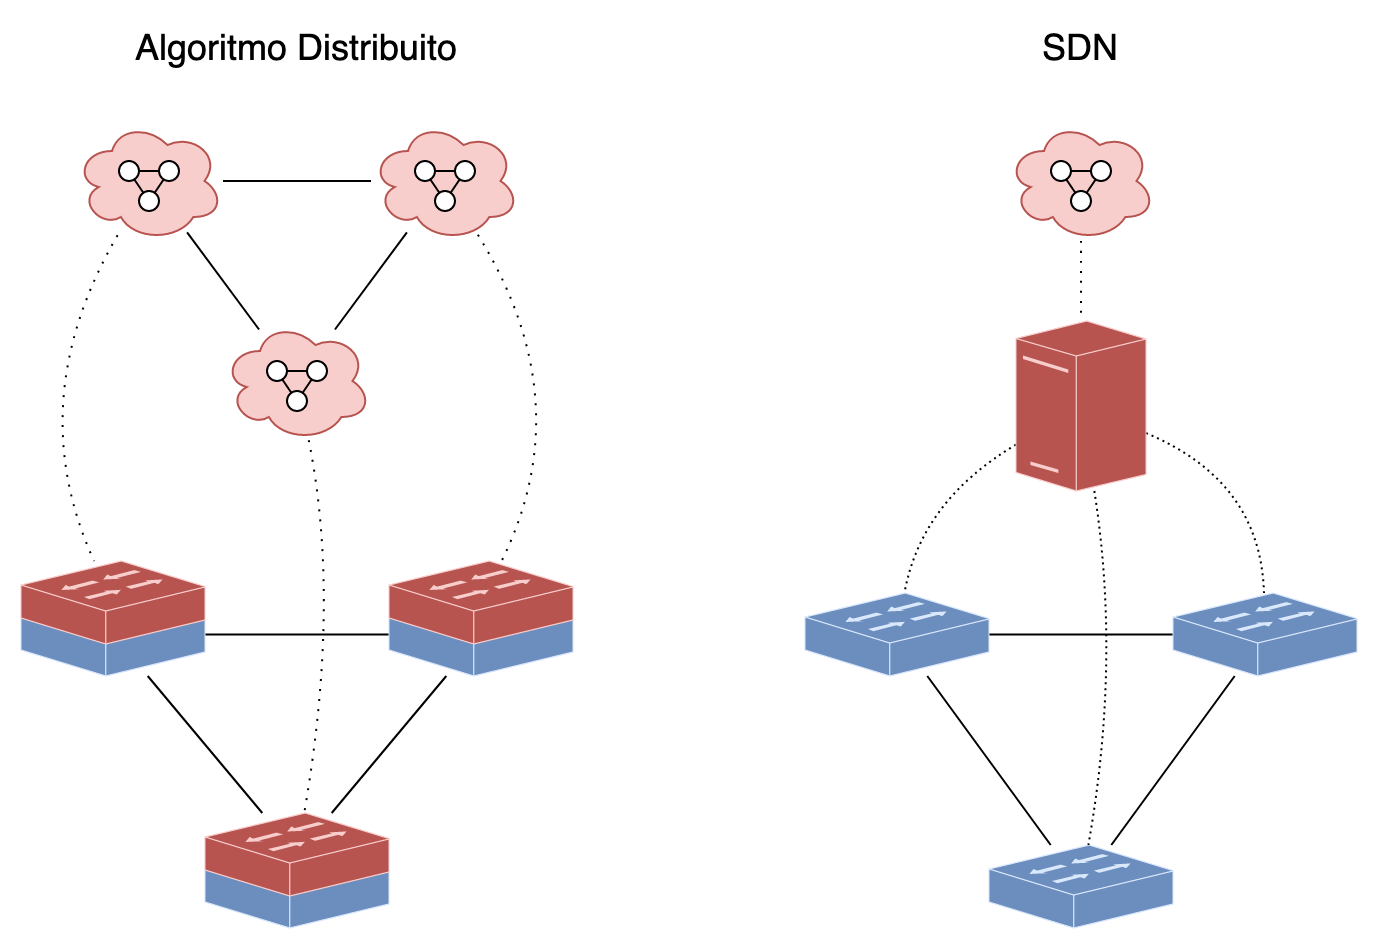
\includegraphics[width=0.7\textwidth]{graphics/trad-vs-sdn.png}
    \caption{Differenza tra approccio tradizionale e SDN}
    \label{fig:trad-vs-sdn}
\end{figure}

Questo approccio, seppur molto valido da un punto di vista teorico, ha dei limiti legati alla difficoltà di realizzare funzioni di complessità crescente e all'impossibilità di convergere rapidamente in caso di guasti. Inoltre è incentrato su valutazioni di tipo topologico e non tiene conto delle condizioni di rete come il livello di congestione di un collegamento che può impattare sull'esperienza d'uso da parte degli utenti, né considera le dinamiche economiche legate alla gestione e alla diversificazione del traffico.

Nell'ultimo decennio, grazie al graduale abbattimento dei costi dell'hardware ed allo sviluppo di soluzioni software sempre più sofisticate, ha preso forma un nuovo modo di costruire le reti, in cui il disaccoppiamento tra data plane e control plane non è più solo logico, ma anche fisico. Si tratta del \textit{Software Defined Networking} (SDN) in cui il data plane è affidato a delle appliance fisiche genericamente chiamate ``switch'' dislocate nei vari nodi, mentre il control plane è centralizzato su server ridondati noti come ``controller'' (\cref{fig:trad-vs-sdn}). La prima soluzione di successo largamente adottata di questo paradigma è OpenFlow, un protocollo aperto che implementa la cosiddetta ``Southbound API'', ossia l'interfaccia di comunicazione tra controllori e switch.

Se da un lato SDN rilassa il legame tra piano dati e di controllo, rimane ancora aperto l'interrogativo su come debba essere realizzato quest'ultimo. Per rispondere a questa domanda, occorre prima individuare i compiti che esso svolge. Oltre a gestire gli algoritmi di instradamento, il control plane si occupa anche di autenticazione ed accounting delle sessioni utente, interconnessione con altre reti, allocazione di risorse per determinati servizi ed in generale tutte quelle forme di governance da cui dipende il transito dei dati sulla rete. A questa dimensione, va aggiunta anche quella delle funzioni della rete e dei servizi che essa offre. Ad esempio si parla di caching dei contenuti tramite le Content Delivery Network (CDN), firewalling, NAT, più tutte le funzioni intermedie necessarie a realizzare architetture più complesse, come quelle proprie della telefonia mobile.

Da questi interrogativi è partita la cordata di 13 grandi operatori Internet che nel 2012 ha dato impulso alla nascita di un segmento di ricerca chiamato \textit{Network Functions Virtualization} (NFV), o virtualizzazione di funzioni di rete \cite{nfvwhitepaper1}. Gli obiettivi erano chiari: superare il modello chiuso imposto dai vendor e realizzare un ecosistema aperto in cui il software del piano di controllo e le relative funzioni potessero risiedere fuori dalle appliance dedicate. Tecnologie di virtualizzazione emergenti come macchine virtuali e container potevano essere sfruttate per ospitare le funzioni su server comuni, meglio conosciuti col nome Commercial Off-The-Shelf (COTS). Un'altra opportunità era rappresentata dai dispositivi ``white box'', router e switch molto veloci risultato del matrimonio tra due realtà: le grandi aziende del silicio, in grado di progettare chip dedicati al data plane, e i produttori di soluzioni integrate. Questa famiglia di device in particolare è sempre più numerosa poiché permette di coniugare prestazioni e flessibilità. Tra i primi ad intraprendere questo percorso vi fu Nvidia che realizzò switch SDN mossi da ASIC Mellanox (poi acquisita) e animati da Cumulus Linux, una distribuzione realizzata ad hoc in grado di mettere a fattor comune merchant silicon con un control plane containerizzato.

\begin{figure}[htb]
    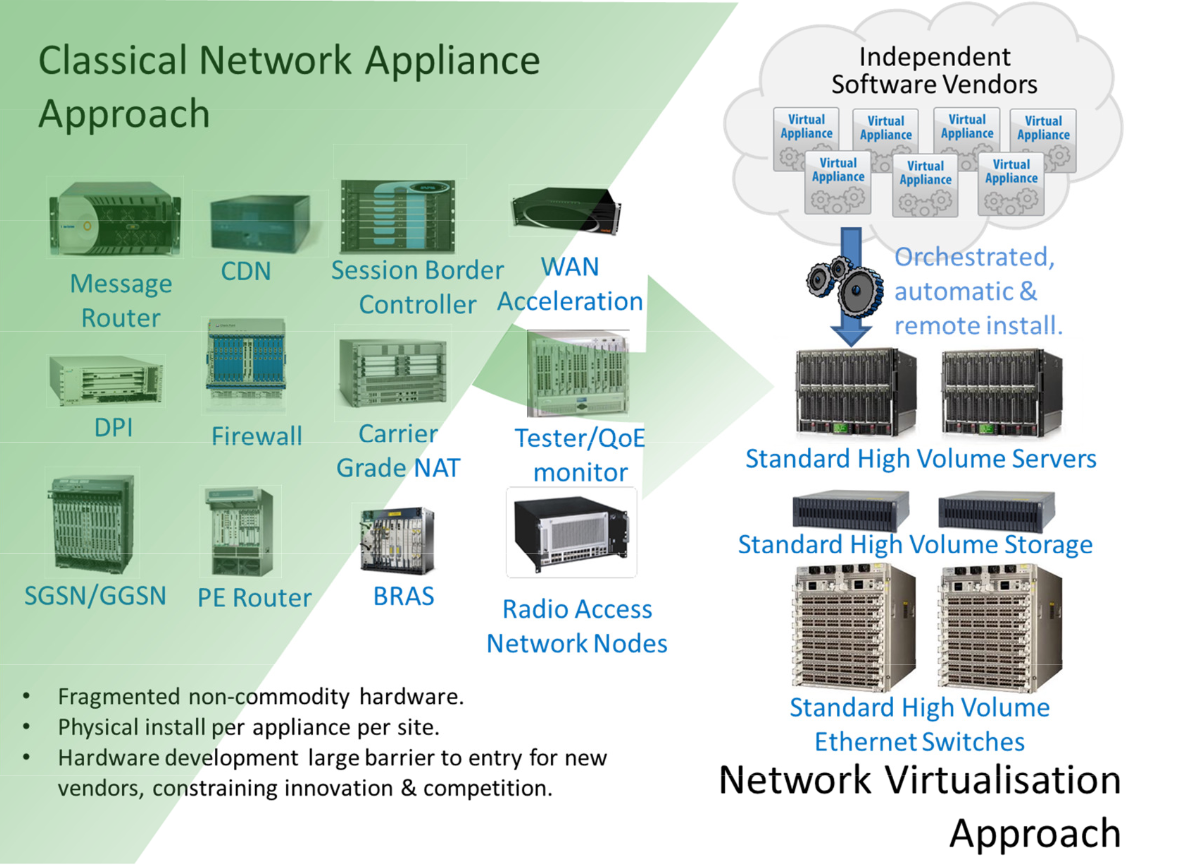
\includegraphics[width=0.7\textwidth]{graphics/trad-vs-nfv.png}
    \caption{Verso NFV}
    \label{fig:trad-vs-nfv}
\end{figure}

Dividere le responsabilità consente di razionalizzare i costi degli apparati fisici, ottimizzare gli investimenti e favorire l'integrazione di soluzioni diverse grazie al contributo dell'open source. L'architettura proposta verrà meglio trattata nel prossimo paragrafo, tuttavia è bene anticipare che le due filosofie, classica e moderna, possono coesistere: ad esempio si può adottare lo stack moderno all'interno dei data center lasciando algoritmi ed apparati tradizionali a gestire le comunicazioni su scala geografica. La divisione tra piano dati e di controllo offre infatti ampi spazi di manovra e lascia al progettista la libertà di implementare l'innovazione senza compromettere quanto di già funzionante esiste nella rete.

\section{ETSI NFV}

L'incipit dei 13 fu raccolto da ETSI, lo European Telecommunications Standards Institute, che creò un Industry Specification Group (ISG) dedicato a NFV con lo scopo di coordinare gli sforzi dei vari operatori: nel giro di pochi anni, infatti, oltre un centinaio di aziende ed enti si dimostrarono interessati all'argomento.

Durante il processo di definizione dei requisiti, ETSI preparò un framework architetturale di riferimento il cui scopo era focalizzarsi sui blocchi funzionali e sui punti di riferimento che sarebbero emersi dalla progettazione della nuova architettura \cite{estinfv002}.

\begin{figure}[htb]
    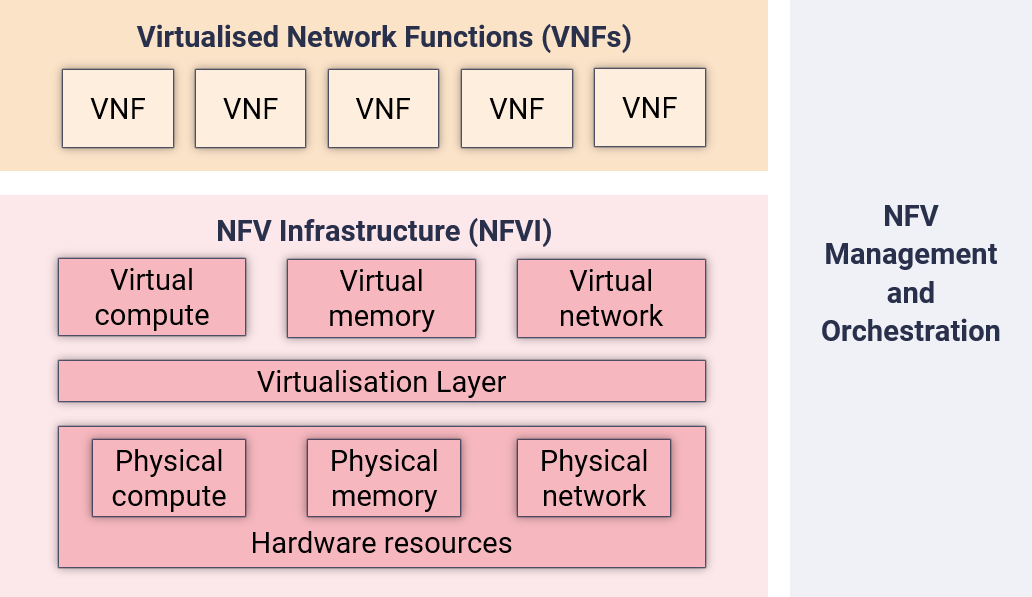
\includegraphics[width=0.7\textwidth]{graphics/high-level_etsi_framework.png}
    \caption{Schema ad alto livello del framework ETSI NFV}
    \label{fig:esti-nfv-high-level}
\end{figure}

Da una visione ad alto livello del lavoro prodotto dal gruppo, si distinguono tre componenti principali (\cref{fig:esti-nfv-high-level}):

\begin{enumerate}
    \item Le Virtualized Network Functions (VNFs), ossia le vere e proprie funzioni del control plane che s'intende virtualizzare. È logico aspettarsi che ognuna di esse sia contraddistinta da dei requisiti, come la necessità di hardware specifico per poter funzionare, ed altre informazioni a corredo.
    \item La NFV Infrastructure (NFVI), cioè le componenti fisiche su cui eseguire le funzioni. Per garantire la flessibilità dell'architettura, le risorse fisiche vengono astratte e presentate alle VNFs sotto forma di risorse virtuali.
    \item NFV Management and Orchestration (MANO), componente trasversale che ha funzioni di controllo sull'architettura, come il monitoring, l'assegnazione delle risorse infrastrutturali alle VNFs e la gestione del loro ciclo di vita.
\end{enumerate}

È importante notare come ciascuno di questi tre blocchi non sia un prodotto finito, ma piuttosto una specifica ad alto livello dei compiti ricoperti dal corrispettivo attore. Non si parla quindi di macchine virtuali o container per le funzioni virtuali, così come non si fa riferimento ad alcun specifico virtualizzatore per l'astrazione delle risorse. Lo stesso vale per la componente di Management and Orchestration di cui però viene fornita un'implementazione di riferimento sotto il nome di \textit{Open Source MANO}.

\begin{figure}[htb]
    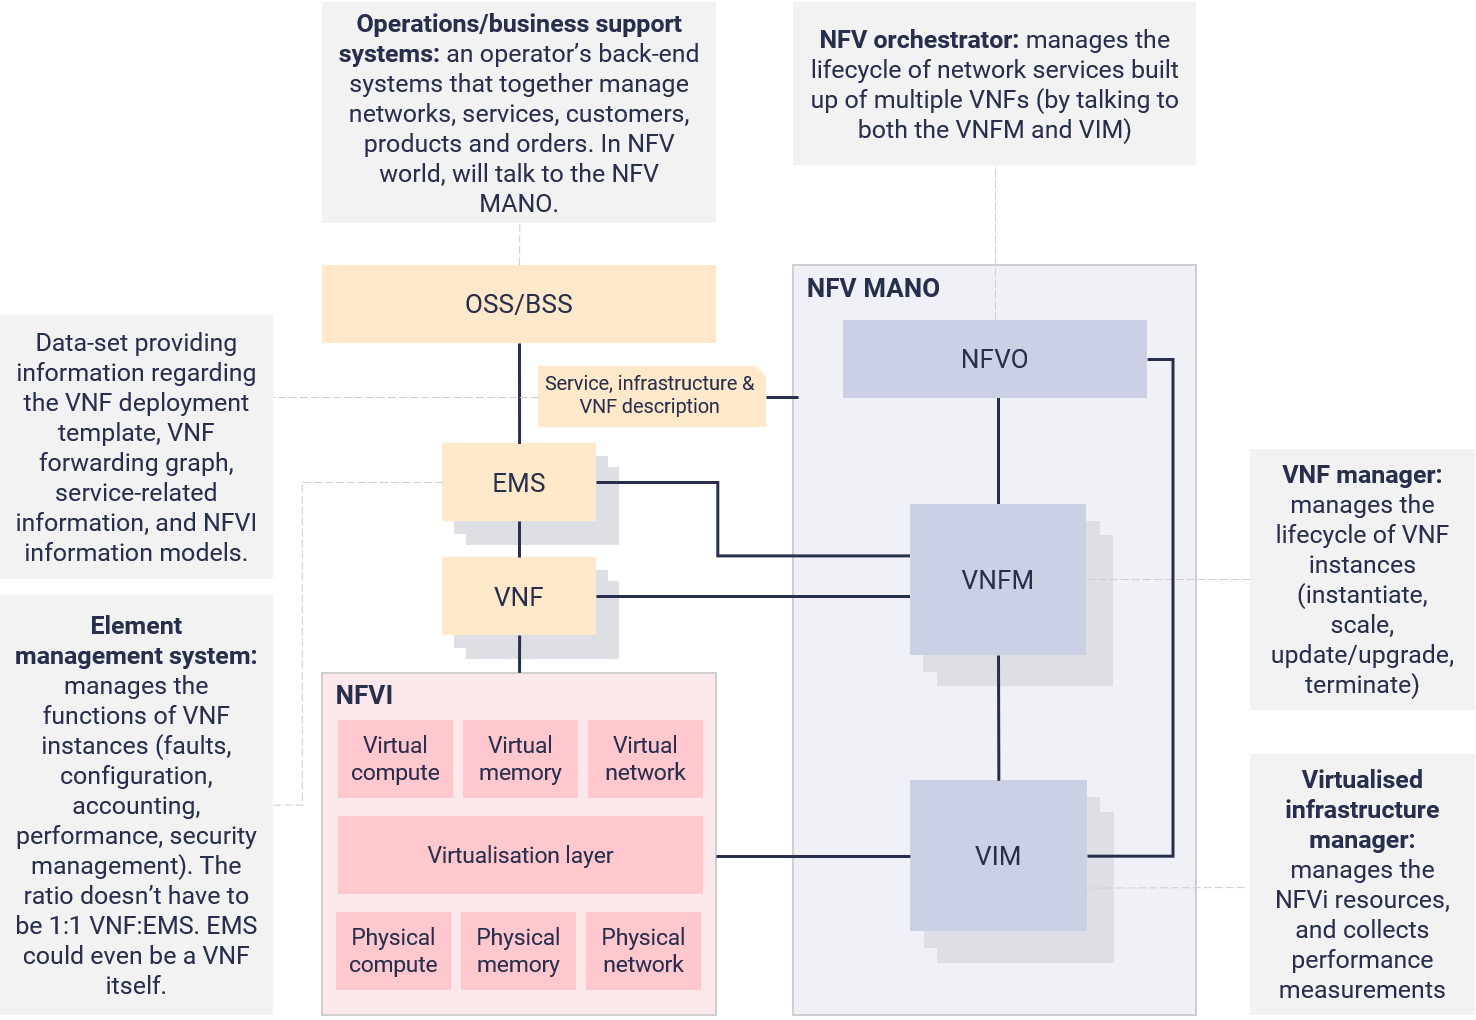
\includegraphics[width=0.7\textwidth]{graphics/full_etsi_framework.png}
    \caption{Schema dettagliato del framework ETSI NFV}
    \label{fig:esti-nfv-low-level}
\end{figure}

La natura agnostica dell'architettura proposta emerge ancor più chiaramente dallo schema dettagliato di ETSI (\cref{fig:esti-nfv-low-level}) dove ciascun blocco funzionale viene spiegato alla luce delle sotto-unità di cui è composto e di come queste comunichino tra loro.

\section{Obiettivi}

L'incipit di questa tesi nasce da un articolo in cui un grande operatore nazionale descrive la nuova architettura della propria rete geografica \cite{revolutiontim}. Questa, come da prassi consolidata, è fisicamente organizzata in anelli simili ad un fiore: al centro si trova la rete core, il pistillo attorno al quale si sviluppano le corone di petali, ossia le reti di trasporto, raccolta e accesso. I vantaggi principali della struttura ad anelli consistono nell'omogeneità progettuale e nell'innata resilienza: da ogni nodo esistono due percorsi per raggiungere lo strato superiore, potendo assicurare un ripiego immediato in caso di guasti.

Dal punto di vista logico ogni livello è caratterizzato da tecnologie diverse. La struttura gerarchica della rete, che concentra il traffico verso il cuore, determina un differenziale nella capacità trasmissiva necessaria, che è minore verso le sedi periferiche e via via crescente verso il livello intermedio di aggregazione e poi verso gli stessi nodi core. Storicamente gli elementi di rete più periferici erano anche i meno sofisticati, fattore che ha contribuito a ridurre i costi data la loro abbondanza. Il risultato è che le reti di accesso e raccolta erano gestite come domini di livello 2 e la ridondanza ottenuta tramite protocolli di spanning tree.

\begin{figure}[htb]
    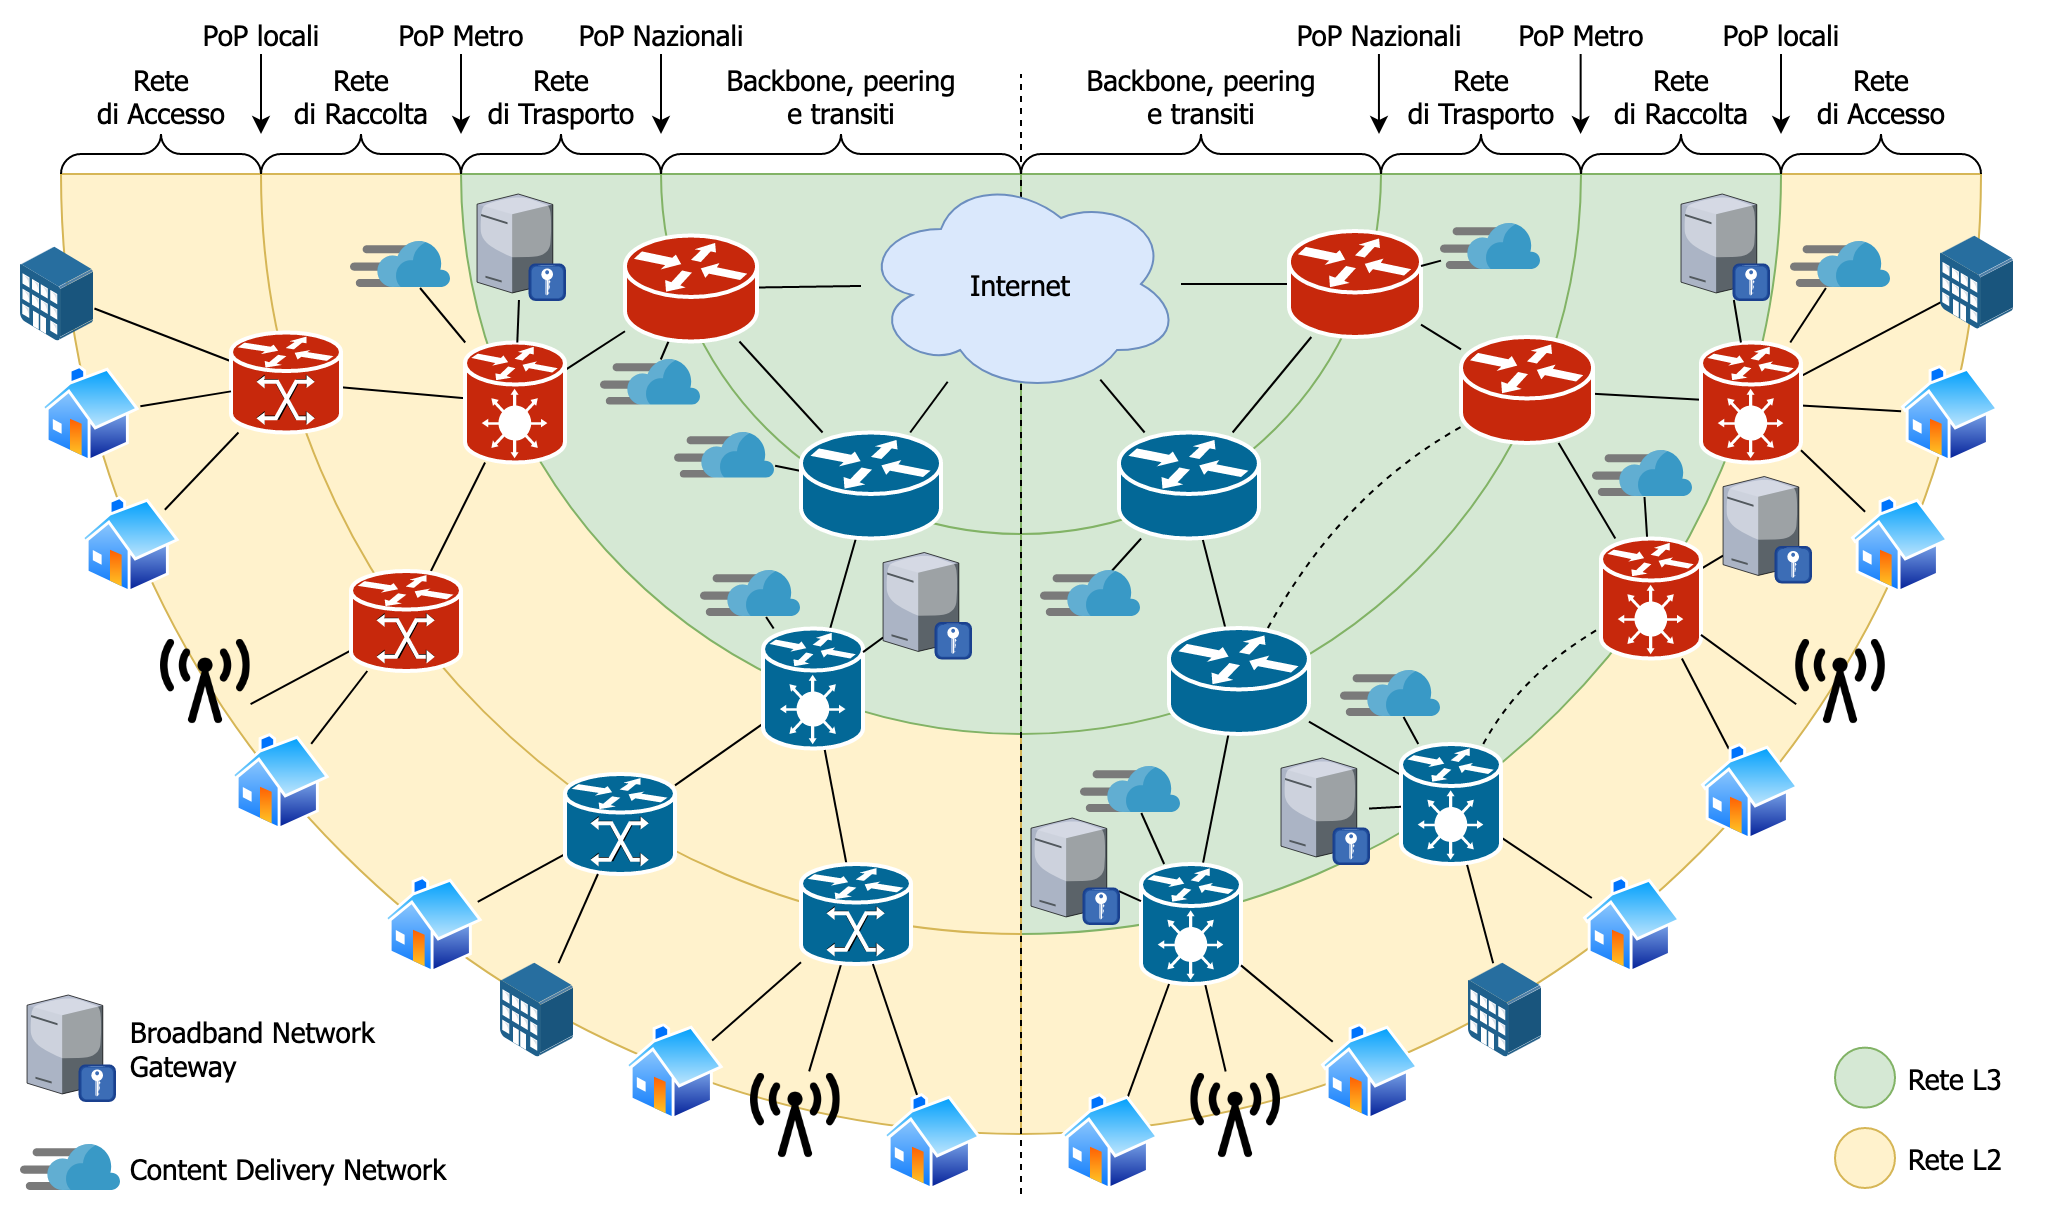
\includegraphics[width=0.8\textwidth]{graphics/isp-arch.png}
    \caption{Le due architetture a confronto}
    \label{fig:isp-arch}
    \begin{adjustwidth}{0.1\textwidth}{0.1\textwidth}
        \centering
        \footnotesize A sinistra lo schema di due reti di accesso e raccolta interamente switchate, a destra un modello con IP fino ai PoP locali. Si noti come nella nuova architettura sia possibile interconnettersi ed erogare servizi all'edge.
    \end{adjustwidth}
\end{figure}

Di recente l'aumento dell'uso di Internet ha definito la necessità di offrire servizi geograficamente vicini agli utenti che altrimenti avrebbero saturato le dorsali per usufruirne: dallo smart working allo streaming sportivo, passando per i contenuti on demand e la rete mobile, la mole di traffico aumenta più velocemente di quanto non progredisca la tecnologia e l'unico modo di stare al passo è distribuire il carico in più punti accorciando altresì la distanza tra domanda e offerta. S'inizia dunque a parlare di \textit{edge computing}, contrapposto alla visione centralizzata. CDN, centralini VoIP e perfino elementi della rete 5G devono trovare posto ai bordi. Per riuscirvi però è necessario rivedere la rete, introducendo il livello IP laddove prima non era presente.

Riprogettare offre l'opportunità unica di sbizzarrirsi e sperimentare nuove idee, partendo da una tela bianca. Perché dunque non immaginare un'architettura completamente virtuale, orchestrata su moderni sistemi software, in cui ogni funzione, ivi compreso il routing, è realizzata su server ad alte prestazioni? A questo punto persino il \textit{peering decentralizzato all'edge su architettura cloud} diventa una prospettiva conquistabile. Nei prossimi capitoli descriverò il nostro tentativo, focalizzando la narrativa sulle tecnologie, sui sistemi, sulle difficoltà riscontrate e sui risultati.